    %!TEX program = lualatex

%==============================================================================
%== template for an LUH LaTeX poster ==========================================
%==============================================================================
%
%--A0 beamer slide-------------------------------------------------------------
\documentclass[english,final,20pt,leqno,print]{beamer}
\usepackage[orientation=portrait,
            size=a0,  % paper size
            scale=1.5 % font scale factor
           ]{beamerposter}

\usepackage{printlen}
\usepackage{subcaption}
\usepackage{adjustbox}
\usepackage{csquotes}
\usepackage{mdframed}


% Uncomment following line, if you have the LUH font rotis installed in `font/rotis/`
\usepackage{fontspec}
%\setmainfont[
%    Path        = font/rotis/,
%    Extension   = .otf,
%    Ligatures   = TeX,
%    BoldFont    = {RotisSansSerifStd-ExtraBold},
%    ItalicFont  = {RotisSansSerifStd-Italic},
%]{RotisSansSerifStd-Regular}

\usepackage{babel}
\usepackage[mode=text]{siunitx}
\usepackage[noabbrev]{cleveref}

\usepackage{tikz}
\usetikzlibrary{shapes, positioning, patterns,matrix,positioning,calc,fit}
\pgfdeclarelayer{background}
\pgfdeclarelayer{foreground}
\pgfsetlayers{background,main,foreground}

\def\imgcoord(#1,#2)(#3){
    \coordinate (#3) at (#1/100,1-#2/100);
}

\def\overlaytextn(#1,#2)(#3)(#4){
	\node[anchor=south,align=center] (text_#3) at (#1,#2) {#4};
	\draw[line width=1mm,line cap=round,color=colorLUHgreen] (text_#3.south) -- (part_#3) circle (2mm);
}
\def\overlaytexts(#1,#2)(#3)(#4){
	\node[anchor=north,align=center] (text_#3) at (#1,#2) {#4};
	\draw[line width=1mm,line cap=round,color=colorLUHgreen] (text_#3.north) -- (part_#3) circle (2mm);
}
\def\overlaytextw(#1,#2)(#3)(#4){
	\node[anchor=east,align=right,text width=5cm] (text_#3) at (#1,#2) {#4};
	\draw[line width=1mm,line cap=round,color=colorLUHgreen] (text_#3.east) -- ++ (0.5,0) -- (part_#3) circle (2mm);
}
\def\overlaytexte(#1,#2)(#3)(#4){
	\node[anchor=west,align=left,text width=5cm] (text_#3) at (#1,#2) {#4};
	\draw[line width=1mm,line cap=round,color=colorLUHgreen] (text_#3.west) -- ++ (-0.5,0) -- (part_#3) circle (2mm);
}

%\linespread{1.15}
%
%==The poster style============================================================
\usetheme[
print % uncomment for RGB color draft settings
]{LUHposter}

\setlength{\leftmargini}{1.5cm}

%==Title, date and authors of the poster=======================================
\title %
[ELGRA Symposium 2024 -- 03.\,--\,06.09.2024 -- Liverpool, United Kingdom] % Conference/occasion of the poster
{% Poster title
An Affordable Autonomous 2U-Greenhouse for Plant Research in Low-Gravity Environments
}

\author{% Authors
\textbf{Dominik Woiwode\texorpdfstring{$^\dagger$}}, \textbf{Jakob Marten\texorpdfstring{$^\ddagger$}}, \normalsize Justin Sondheim, Dörthe Behrens, Nils Wörz, Natalija Hohnjec, Helge Küster, Holger Blume 
}

\institute
[Leibniz University Hannover] % University
{
Leibniz University Hannover, \small $^\dagger$Institute for Information Processing, $^\ddagger$Institute of Microelectronic Systems
}
\date{\today}

% Logo of the institute, if any
\institutelogo{
\includegraphics[height=\luhlogoheight]{img/logo/Logo_Gluecksklee_1024}\hspace{2cm}
\includegraphics[height=\luhlogoheight]{img/logo/TNT_darkv4.png}\hspace{2cm}
\includegraphics[height=\luhlogoheight]{img/logo/IMS_Logo_transparent.png}}

\begin{document}

\begin{frame}[t]
\begin{center}%
\raggedright
{\color{colorLUHtitleblue}\fontsize{100}{90}\selectfont{\bfseries \inserttitle{}}\\[1ex]}
{\Large{\insertauthor}\\[0.7ex]}
{\normalsize{\insertinstitute}}
\end{center}
\vspace{0.5\verticalspacing}
%==============================================================================
\begin{columns}[T]
%==============================================================================
%==The poster content==========================================================
%==============================================================================

% First column
\begin{column}{.49\textwidth}
  \begin{block}{\strut{}\textbf{Motivation \& Purpose}}
    \begin{itemize}
      \item 2U-Greenhouse for plant experiments in low gravity
      \item Low material costs (<500€) due to commercial of the shelf (COTS) parts
      \item Designed as part of the Überflieger2 contest for the investigating of root nodule symbiosis between \textit{Medicago truncatula} and \textit{Sinorhizobium meliloti} on the International Space Station (ISS)~\textcolor{colorLUHblue}{\cite{biospektrum}}
    \end{itemize}
  \end{block}


  \begin{block}{\strut{}\textbf{Setup of the Greenhouse}}
  \vspace{-.85em}
    \begin{figure}
    \vspace{-.85em}
        \centering
        \begin{tikzpicture}[font=\scriptsize]
            \def\xstart{0}
            \def\xend{0.7\textwidth}
			\begin{pgfonlayer}{background}
				\node[anchor=south west,inner sep=0] (image) at (0,0)
				{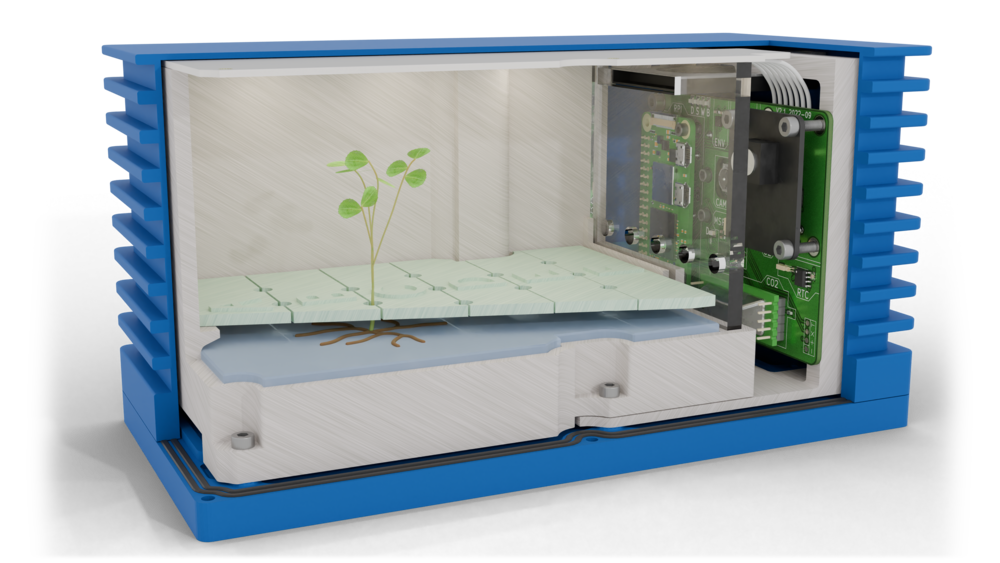
\includegraphics[width=0.7\textwidth]{img/cube_small.png}};
			\end{pgfonlayer}
			\begin{scope}[x={(image.south east)},y={(image.north west)}]
				\imgcoord(20.89,12.41)(part_leds);
				\imgcoord(27.66,26.94)(part_biochamber);
				\imgcoord(30.78,50.56)(part_perforated_plates);
				\imgcoord(34.17,62.96)(part_media);
				\imgcoord(20.10,92.50)(part_cube);
    
				\imgcoord(83.70,14.35)(part_electronic_section);
				\imgcoord(66.88,14.63)(part_fan);
				\imgcoord(73.54,35.28)(part_window);
				\imgcoord(80.57,54.63)(part_mainboard);
				\imgcoord(68.23,75.28)(part_gasket);
			\end{scope}

            \def\ystart{1.25}
            \def\ystep{3}
   
            \overlaytextw(\xstart,\ystep*4+\ystart)(leds)(Light Module);
            \overlaytextw(\xstart,\ystep*3+\ystart)(biochamber)(Bio Chamber);
            \overlaytextw(\xstart,\ystep*2+\ystart)(perforated_plates)(Perforated\\ Plate);
            \overlaytextw(\xstart,\ystep*1+\ystart)(media)(Plant Medium);
            \overlaytextw(\xstart,\ystep*0+\ystart)(cube)(2U Cube);

            \overlaytexte(\xend,\ystep*4+\ystart)(electronic_section)(Electronics\\ Section);
            \overlaytexte(\xend,\ystep*3+\ystart)(fan)(Fan);
            \overlaytexte(\xend,\ystep*2+\ystart)(window)(Window);
            \overlaytexte(\xend,\ystep*1+\ystart)(mainboard)(Mainboard);
            \overlaytexte(\xend,\ystep*0+\ystart)(gasket)(Gasket);
		\end{tikzpicture}
        \caption{Setup of the greenhouse in a 2U cube.}
        \label{fig:cad}
    \end{figure}

    \begin{itemize}
        \item Two separate components (bio chamber, electronics section) in 2U cube
        \item 3D printed (SLA) autoclavable parts using bio-compatible resin
        \item $\num{150}\times\num{94}\times\num{87}$\,\unit{\cubic\mm} volume for plants and plant medium
        \item Fully autonomous operation with self-recoverable software design
        \item Perforated plates shade roots from excessive illumination
        \item Fan to accelerate the diffusion of produced gases necessary due to the lack of convection
    \end{itemize}
    \end{block}

    
    \begin{block}{\strut{}\textbf{Electronics}}
    \vspace{-.15em}
    \begin{figure}
        \vspace{-.15em}
        \centering
        \begin{tikzpicture}[font=\scriptsize]
            \def\xstart{0}
            \def\xend{26.5}
			\begin{pgfonlayer}{background}
				\node[anchor=south west,inner sep=0] (image_1) at (1,0)
				{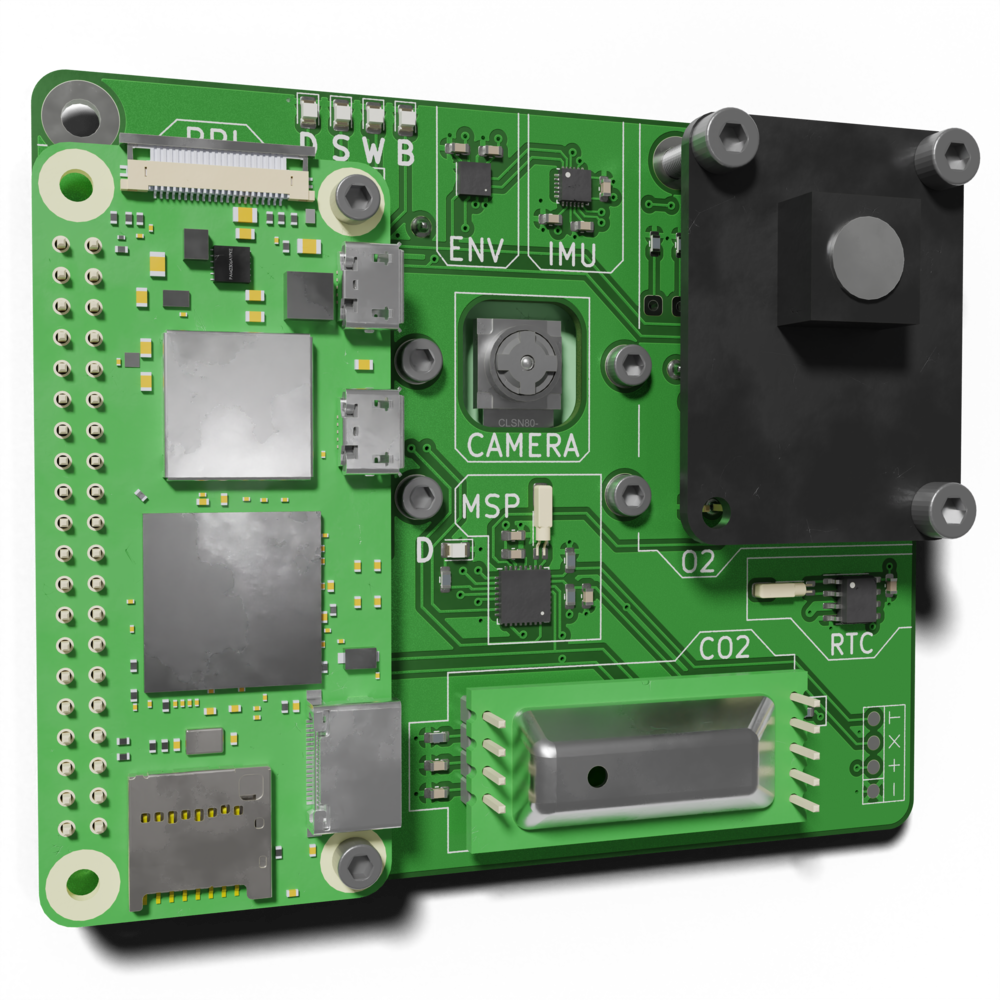
\includegraphics[height=0.43\textwidth]{img/cube_mainboard_small.png}};
    
				\node[anchor=south west,inner sep=0] (image_2) at (17,0)
				{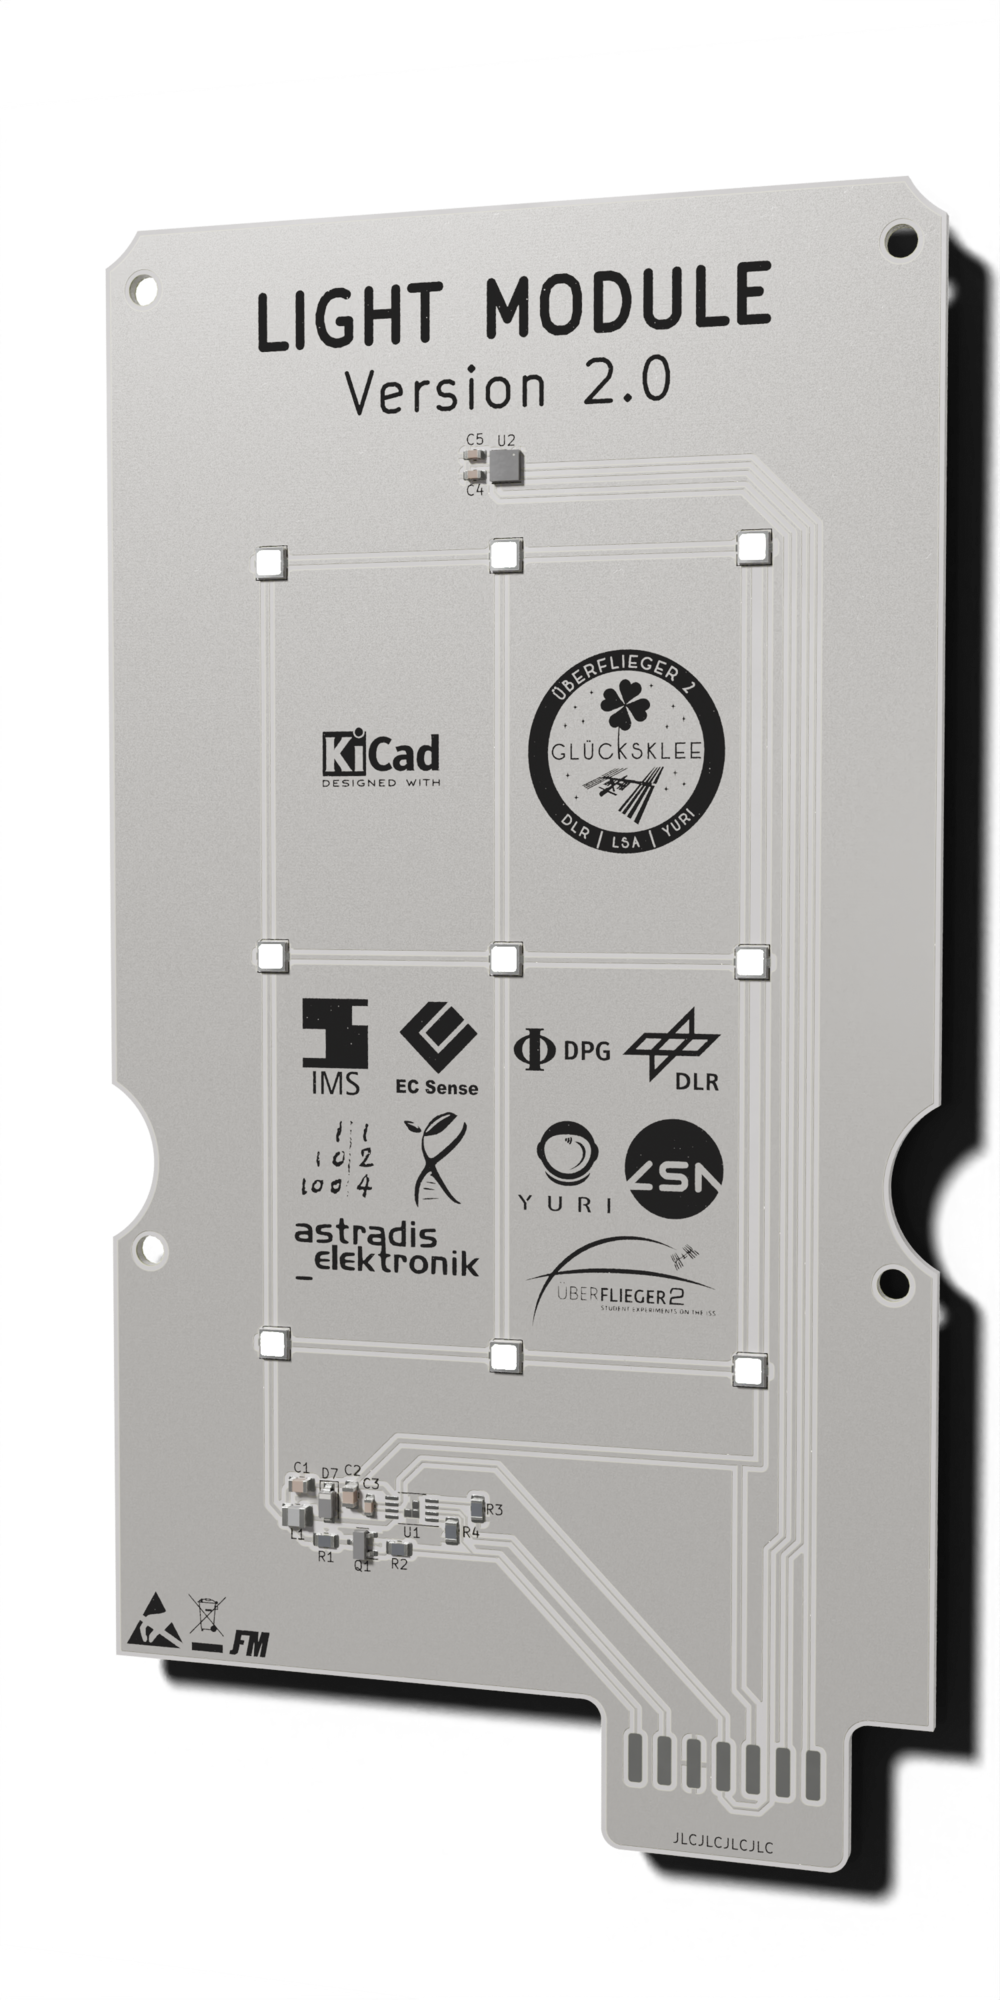
\includegraphics[height=0.43\textwidth]{img/cube_light_small.png}};
			\end{pgfonlayer}
			\begin{scope}[x={(image_1.south east)},y={(image_1.north west)}]
				\imgcoord(23.50,59.30)(part_raspberry);
				\imgcoord(50.20,37.90)(part_camera);
				\imgcoord(55.20,75.50)(part_co2);
				\imgcoord(46.50,17.60)(part_env_1);
				\imgcoord(57.30,19.10)(part_imu);
				\imgcoord(85.40,61.00)(part_rtc);
				\imgcoord(86.70,28.10)(part_o2);
				\imgcoord(30.80,10.70)(part_debug);
				\imgcoord(52.40,59.50)(part_msp);
			\end{scope}
            \begin{scope}[shift={(17,0)},x={(image_2.south east)},y={(image_2.north west)}]
                \imgcoord(49.80,23.53)(part_env_2);			
                \imgcoord(50.60,67.77)(part_led);
				\imgcoord(41.27,75.60)(part_led_controller);
			\end{scope}i

            \def\ystart{1.25}
            \def\ystep{2.7}

            \overlaytextw(\xstart,\ystep*5+\ystart)(debug)(Debug);
            \overlaytextw(\xstart,\ystep*4+\ystart)(env_1)(Temperature\\ Humidity);
            \overlaytextw(\xstart,\ystep*3+\ystart)(camera)(Camera);
            \overlaytextw(\xstart,\ystep*2+\ystart)(raspberry)(Raspberry Pi Zero 2W);
            \overlaytextw(\xstart,\ystep*1+\ystart)(msp)({MSP430\\ Microcontroller});
            \overlaytextw(\xstart,\ystep*0+\ystart)(co2)(Carbon Dioxide);

            \overlaytexte(\xend,\ystep*5+\ystart)(imu)(Acceleration);
            \overlaytexte(\xend,\ystep*4+\ystart)(env_2)(Temperature Humidity);
            \overlaytexte(\xend,\ystep*3+\ystart)(o2)(Oxygen);
            \overlaytexte(\xend,\ystep*2+\ystart)(rtc)(Real-Time Clock);
            \overlaytexte(\xend,\ystep*1+\ystart)(led)({Light Emitting Diode (LED)});
            \overlaytexte(\xend,\ystep*0+\ystart)(led_controller)(LED-Controller);
		\end{tikzpicture}
        \caption{Mainboard (left) and Light Module (right) used in the greenhouse.}
        \label{fig:boards}
    \end{figure}
    
    \begin{itemize}
        \item Raspberry Pi Zero 2W as main processor with MSP430 microcontroller
        \item Different sensors for monitoring temperature, humidity, oxygen, carbon dioxide and acceleration; camera for image and video footage
        \item Communication via Ethernet-over-USB interface to main payload
        \item Designed for shared atmosphere for simpler sensor placement
        \item Real-time clock for timekeeping during (ground) operation and launch
    \end{itemize}
    %\end{block}
     
    %\begin{block}{\strut{}\textbf{Literature}}
    \vspace{3.2em}
    \hrule
    
    %\begin{mdframed}
    \begin{thebibliography}{99}
      \bibitem{biospektrum} N. Wörz, J. Sondheim, D. Behrens, D. Woiwode, D. Rudy, and Team Glücksklee, ‘Pflanzenforschung an Bord der ISS’, \\BIOspektrum, vol. 29, no. 5, pp. 557–557, Sep. 2023, https://doi.org/10.1007/s12268-023-1972-1
    \end{thebibliography}
    %\end{mdframed}
    \end{block}    
\end{column}

%Second Column
\begin{column}{.49\textwidth}

  \begin{block}{\strut{}\textbf{Software}}
  \begin{itemize}
    \item Main purpose: control light and fan in regular cycles; secondary purpose: gather sensor data and camera footage
    \item Implemented using Python 3 on Raspberry Pi OS
    \item Independent modules that stay functional if another fails
    \item Built-in failure recovery with MSP430: If a heartbeat signal is not received within one minute, the microcontroller attempts to restart the Raspberry Pi Zero 2W and therefore the software
  \end{itemize}
  \end{block}


  \begin{block}{\strut{}\textbf{Mission Findings}}
\begin{figure}
\begin{minipage}[c]{0.49\textwidth}
\vspace{-26pt}
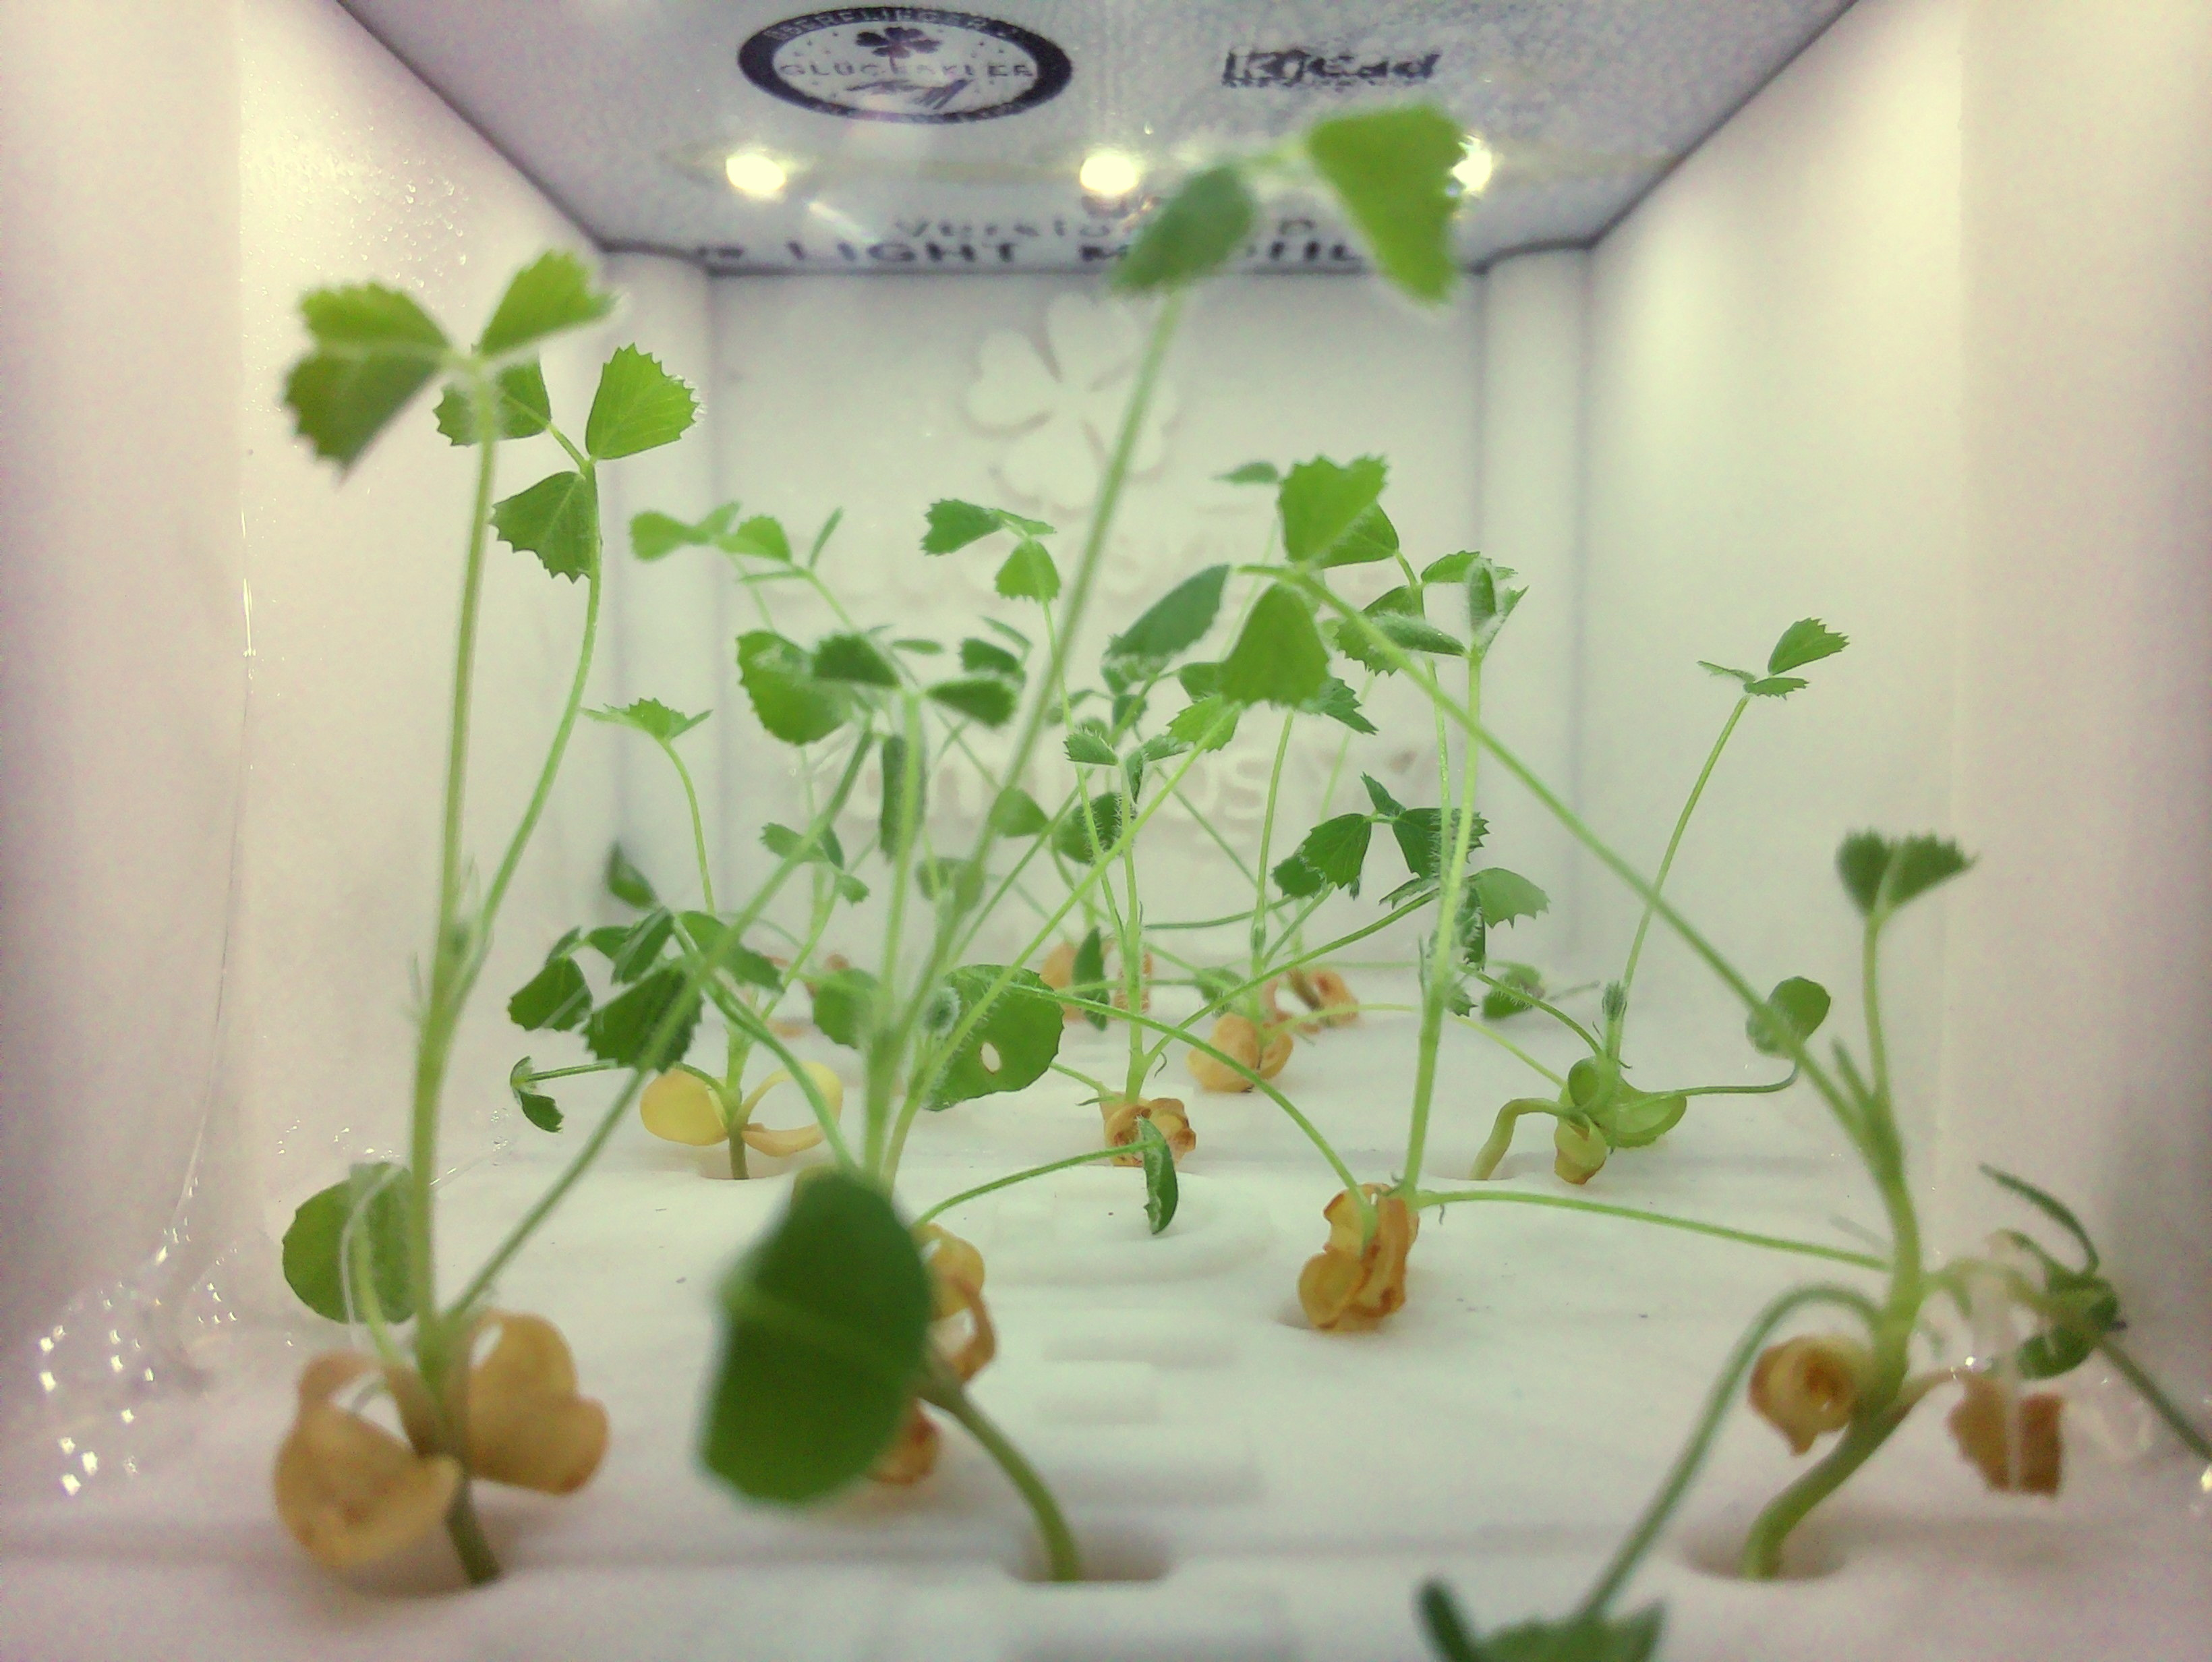
\includegraphics[width=\textwidth]{img/experiment_edit.jpeg}
\caption{View from inside the experiment.}
\end{minipage}
\hfill
\begin{minipage}[c]{0.49\textwidth}
\vspace{10pt}
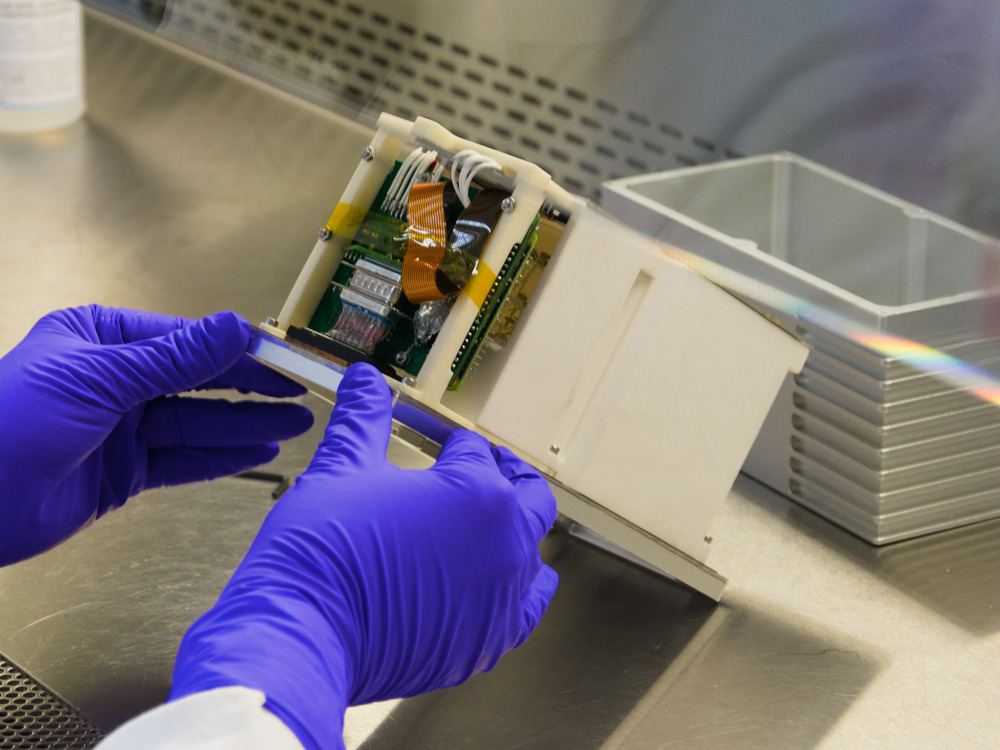
\includegraphics[width=\textwidth]{img/DSC_5297_edited_blue_small.jpg}
\caption{Experiment during assembly in sterile bench.}
\end{minipage}%
\end{figure}

  \begin{itemize}
    \item Was actively operated for 22 days during SPX-27 mission on the ISS
    \item As expected, the high humidity caused problems for some sensors
    \item Hardware and software continued to run successfully, maintaining the fan and light cycles despite sensor failures
    \item Loss of data during launch operation due to misconfiguration, causing the memory to fill up
    \item Average power consumption: \qty{900}{mW} (day), \qty{780}{mW} (night) 
    \item Gas values show an active photosynthesis cycle which lines up with day-night-cycle
  \end{itemize}
  
  \begin{figure}
    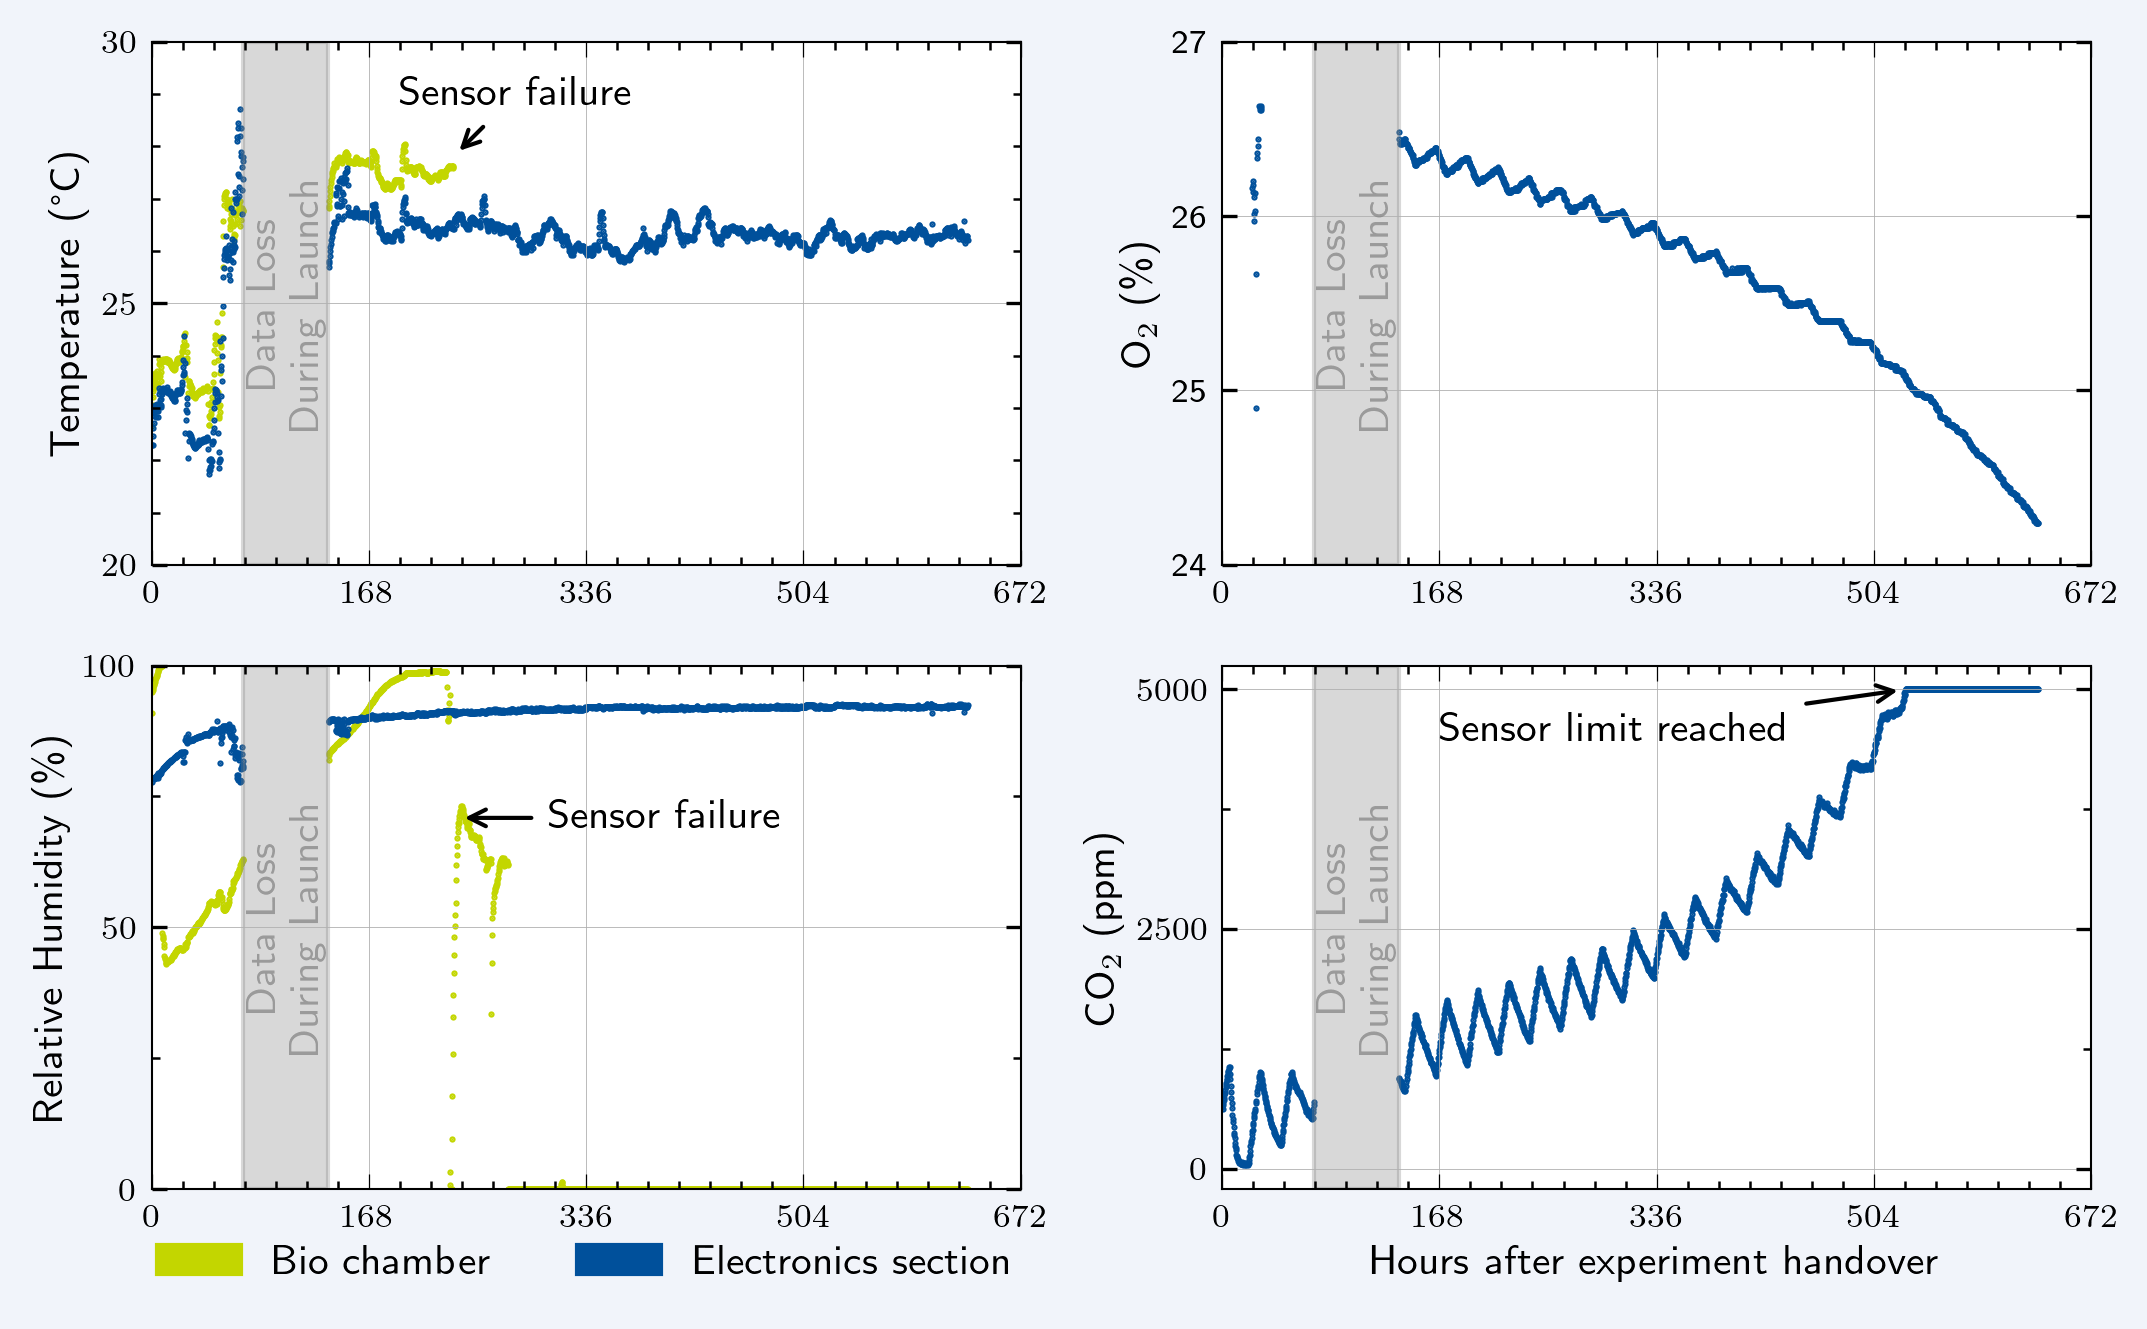
\includegraphics[width=\textwidth]{img/elgra_plot_2_2.png}
    %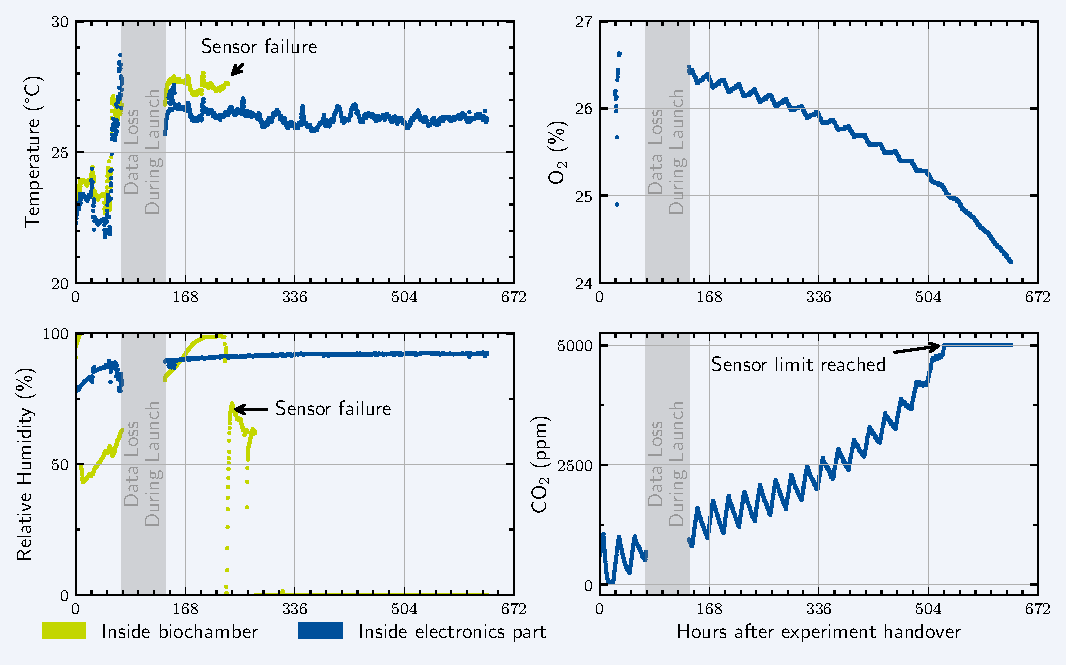
\includegraphics[width=\textwidth]{img/elgra_plot_2_2_facecolor.pdf}
    \caption{Sensor measurements from selected sensors during SPX-27 mission on ISS.}
    \label{fig:sensor_data}
  \end{figure}
\vspace{-1.5em}
  \end{block}

  \begin{block}{\strut{}\textbf{Acknowledgements}}
    \begin{itemize}
        \item German Aerospace Center (DLR) for sponsoring the Überflieger2 contest
        \item Institute of Plant Genetics (Section IV - Plant Genomics) for providing a laboratory and scientific supervision
        \item yuri GmbH for organizational and technical supervision and support
        \item All our sponsors who helped during the project
    \end{itemize}
  \end{block}

\end{column}

\end{columns}

%==============================================================================
\end{frame}
\end{document}